\documentclass[a4paper]{article}

\usepackage[utf8]{inputenc}
\usepackage[T1]{fontenc}
\usepackage{graphicx}
\usepackage{hyperref}
\usepackage{amsmath}
\usepackage{amssymb}
\usepackage{mathenv}
\usepackage{multirow}

\DeclareMathAlphabet{\itbf}{OML}{cmm}{b}{it}

% numérotation au sein de chaque section (du style "2.1")
\numberwithin{equation}{section}

% commandes perso
\newcommand{\R}{\mathbb{R}}
\newcommand{\N}{\mathbb{N}}
\newcommand{\C}{\mathcal{C}}

\newcommand{\bnu}{{\boldsymbol{\nu}}}

\title{Consistency of Fanbeam Projections Along an Arc of a Cycloid}
\author{}
\date{}

\begin{document}

\maketitle

\begin{abstract}
This note aims at extending the results of~\cite{clackdoyle2015consistency} to the case of an arc of cycloid, instead of an arc of circle.
\end{abstract}

\section{Introduction}

Let us begin with some notations. The reader shall refer to Figure~\ref{fig:notations}, which is analogous to~\cite[Figure~2]{clackdoyle2015consistency}. The object to be imaged in given by its density function $\mu(x)$ and is illuminated by a source that follows an arc of cycloid. In other words, the fanbeam projection data $g(t,\gamma)$ is given by
\begin{equation}
	g(t,\gamma) = \int_0^{+\infty} \mu \left( s(t) + l \left[ \sin (\gamma + \lambda_t), -\cos (\gamma + \lambda_t) \right] \right) dl
\end{equation}
The cycloid is parametrized by $t$ in the following way
$$
s(t) = \left( -R_0 \sin(\omega t) - \left( t + \frac{T}{2} \right) v, R_0 \cos(\omega t) \right),
$$
where $R_0$, $\omega$ and $v$ are fixed constants.
\begin{figure}[!ht]
	\centering
	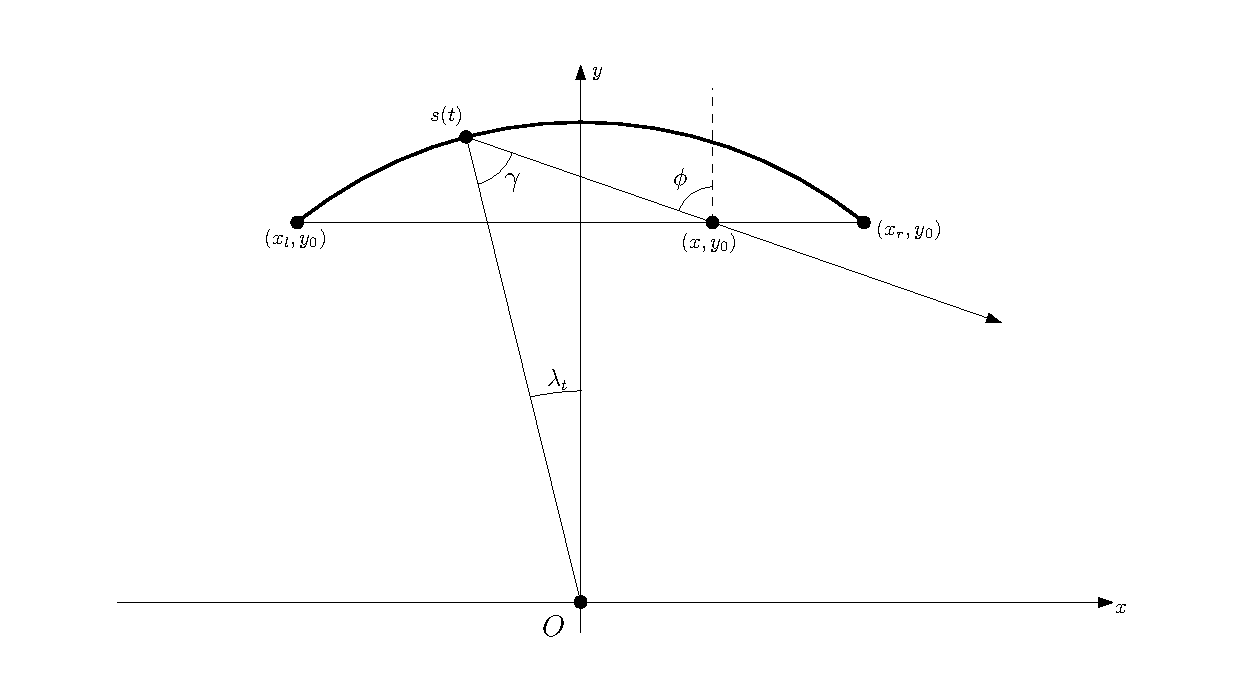
\includegraphics[width=13cm]{figure.eps}
	\caption{Problem under consideration. The source point $s(t)$ follows the cycloid depicted in bold, and the virtual point has coordinates $(x,y_0)$.\label{fig:notations}}
\end{figure}

We will denote $R_t$ the distance between the center $O$ and the source point $s(t)$, and $\lambda_t$ the angle formed with the $y$-axis. Namely, one has
\begin{align}
R_t &= \sqrt{ \left( R_0 \sin(\omega t) + tv \right)^2 + R_0^2 \cos^2(\omega t) }, \\
\lambda_t &= \arctan \left( \frac{R_0 \sin(\omega t) + tv}{R_0 \cos(\omega t)} \right).
\end{align}

\section{Derivation of DCCs}

The DCCs derived in~\cite{clackdoyle2015consistency} heavily rely on a relation between $\tan \phi$ and the angle $\lambda_t$, which is then differentiated to change variables into the following integral
\begin{equation}
	B_n(x) = \int_{-\pi/2}^{\pi/2} g_v(x,\phi) \frac{\tan^n \phi}{\cos \phi} d\phi,	
	\label{eq:Bn_x_phi}
\end{equation}
where $g_v(x,\phi)$ is the virtual fanbeam projection whose virtual source is located at $(x,y_0)$. In other words,
\begin{equation}
	g_v(x,\phi) = \int_0^{\infty} \mu\left( (x,y_0) + l(\sin \phi, -\cos \phi) \right) dl.
\end{equation}

We will follow the same path in this note. First, the formula giving $\tan \phi$ is nearly the same as in~\cite{clackdoyle2015consistency}, \emph{i.e.}
$$
\tan \phi = \frac{x + R_0 \sin(\omega t) + tv}{R_0 \cos(\omega t) - y_0}
$$
Then, taking its derivative allows us to write the Jacobian for a change of variables from $\phi$ to $t$
\begin{align*}
\frac{d\phi}{\cos^2 \phi} &= \frac{ \left( R_0 \omega \cos(\omega t) +v \right) \left( R_0 \cos(\omega t) - y_0 \right) + R_0 \omega \sin(\omega t) \left( x + R_0 \sin(\omega t) + tv \right) }{ \left( R_0 \cos(\omega t) - y_0 \right)^2 } dt \\
 &= \frac{ R_0^2 \omega - v y_0 + R_0 \cos(\omega t)(v-\omega y_0) + R_0 \omega \sin(\omega t)(x +tv) }{ \left( R_0 \cos(\omega t) - y_0 \right)^2 } dt\\
 &:= J(x,t) dt.
\end{align*}
Hence, one can write
\begin{align}
	\frac{\tan^n \phi}{\cos \phi} d\phi &= \tan^n \phi \cos \phi \frac{d\phi}{\cos^2 \phi} \\
	&= \frac{ \left( x+R_0 \sin(\omega t) + tv \right)^n }{D_{x,t} \left( R_0 \cos(\omega t) - y_0 \right)^{n-1}} J(x,t) dt \label{eq:Dxt_first_occurence} \\
	&:= W_n(x,t) dt,
\end{align}
where the term $D_{x,t}$ in equation~(\ref{eq:Dxt_first_occurence}) refers to the distance between the source point $s(t)$ and the virtual point $(x,y_0)$.
In any case, equation~(\ref{eq:Bn_x_phi}) can be re-written as
\begin{equation}
	B_n(x) = \int_{-T/2}^{T/2} g(t,\gamma) W_n(x,t) dt,
\end{equation}
where $T$ is defined such that $s(-T/2) = \left(x_r,y_0\right) $ and $s(T/2) = \left(x_l,y_0\right)$. Note that the angle $\gamma$ depends on $x$ and $t$ in the following way
\begin{equation}
	\cos \gamma = \frac{\left(R_0 \sin (\omega t) + tv \right) \left(x + R_0 \sin (\omega t) + tv \right) - R_0 \cos (\omega t) \left( y_0 - R_0 \cos(\omega t) \right)}{R_t D_{x,t}}.
\end{equation}

\section{Numerical simulations}

To be continued.

\bibliographystyle{plain}
\bibliography{DCC_cycloid}

\end{document}

